\RequirePackage{plautopatch}
\documentclass[upLaTeX,a4paper]{jsarticle}
\usepackage{listings,jlisting,amsmath,otf,here,empheq}
\usepackage[dvipdfmx]{graphicx}

\lstset{
breaklines = true,
numbers = left,
frame = tbrl,
tabsize = 4,
captionpos = t
}

\title{流体の数値計算プログラムの作成 中間報告}
\author{B4 津田修一朗}
\date{2021/5/31}

\begin{document}
\maketitle

\section{これまでに取り組んだこと}
\subsection{環境構築}
gfortranとgnuplotをインストールした.
エディタはVisual Studio Codeを使用している.


\subsection{流れ関数と渦度を求めるプログラムの実装}
流れ関数-渦度法により,cavity内の流れを解いた.基礎方程式については\cite{1}に従った.レイノルズ数$Re = 50$, 格子点$50\times 50$とした.

\subsection{速度ベクトル図の描画}
流れ関数と渦度を求めるプログラムの実装により得られた流れ関数$\phi$より,速度場$(u, v)$を

\begin{equation}
  u = \frac{\partial \phi}{\partial y}, v = - \frac{\partial \phi}{\partial x},
\end{equation}
を用いて求めた.
ただし,u, vの境界条件は
\begin{empheq}{alignat=2}
  u = -1, v = 0 \quad 移動壁上 \\
  u = 0, v = 0 \quad 静止壁上
\end{empheq}
とした.
図\ref{fig:velocity_vector}に今回得られた速度ベクトル図を示す.図\ref{fig:velocity_vector}より,$(0,1),(1,1)$間を結ぶ線分に相当する移動壁面付近で比較的速い流れが生じ,cavity内に1つの渦ができていることが確認できる.
\begin{figure}[H]
  \centering
  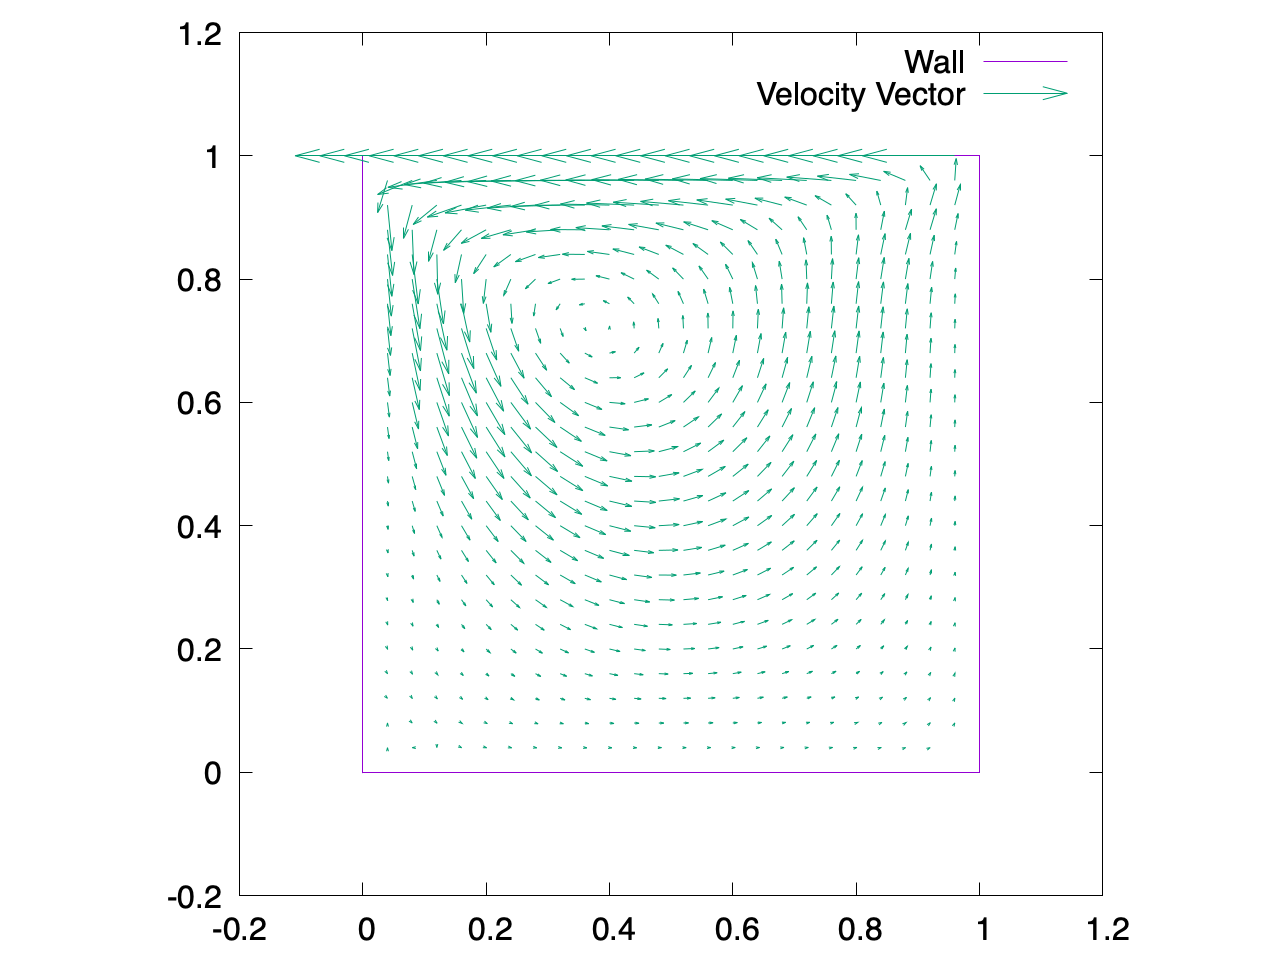
\includegraphics[width=15cm]{outputs/img/velocity_vector.png}
  \caption{速度ベクトル}
  \label{fig:velocity_vector}
\end{figure}

\section{現在取り組んでいること}
\subsection*{流線図の描画}
流線は流れ関数$\phi = const$で表されることを用いて,流れ関数と渦度を求めるプログラムにより求めた流れ関数を用いて流線図の描画を行った.
その結果を図\ref{fig:stream_line_wo_param}に示す.この時、gnuplotのdgrid3d機能を用いて描画を行ったが、格子点数と比較して描画に用いる点の数が少なく,滑らかな流線が得られなかった。さらに、流線が壁で途切れ、不自然によどみ点となっている箇所も複数あった。この原因は、dgrid3dは非格子状データから格子状データへ変換を行うものであり、
その際に複数の異なる点の重み付き平均をとっていること\cite{2}が原因と考えた。そのため、dgrid3dが生成する格子数を数値解析と同じにし、遠い点の影響が少なくなるように重みのパラメータを調整した。その結果を図\ref{fig:stream_line}に示す。図\ref{fig:stream_line}では、図\ref{fig:stream_line_wo_param}でみられた問題点は解消されている。
今後はさらに良い方法が無いか検討するとともに、グラフの整形等も行う。
\begin{figure}[H]
  \centering
  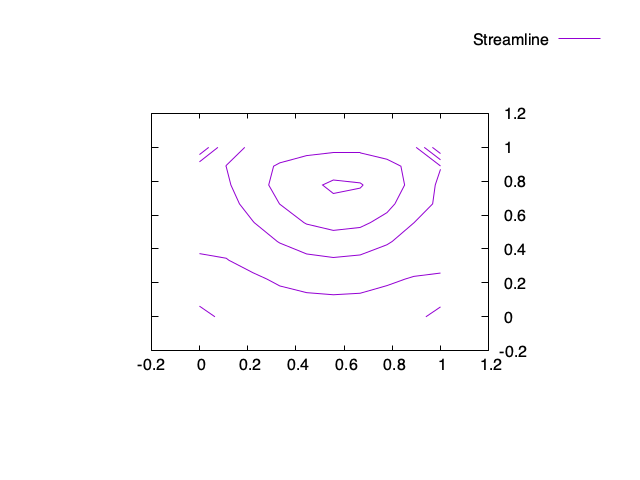
\includegraphics[height=9.5cm]{outputs/img/stream_line_wo_param.png}
  \caption{流線}
  \label{fig:stream_line_wo_param}
\end{figure}
\begin{figure}[H]
  \centering
  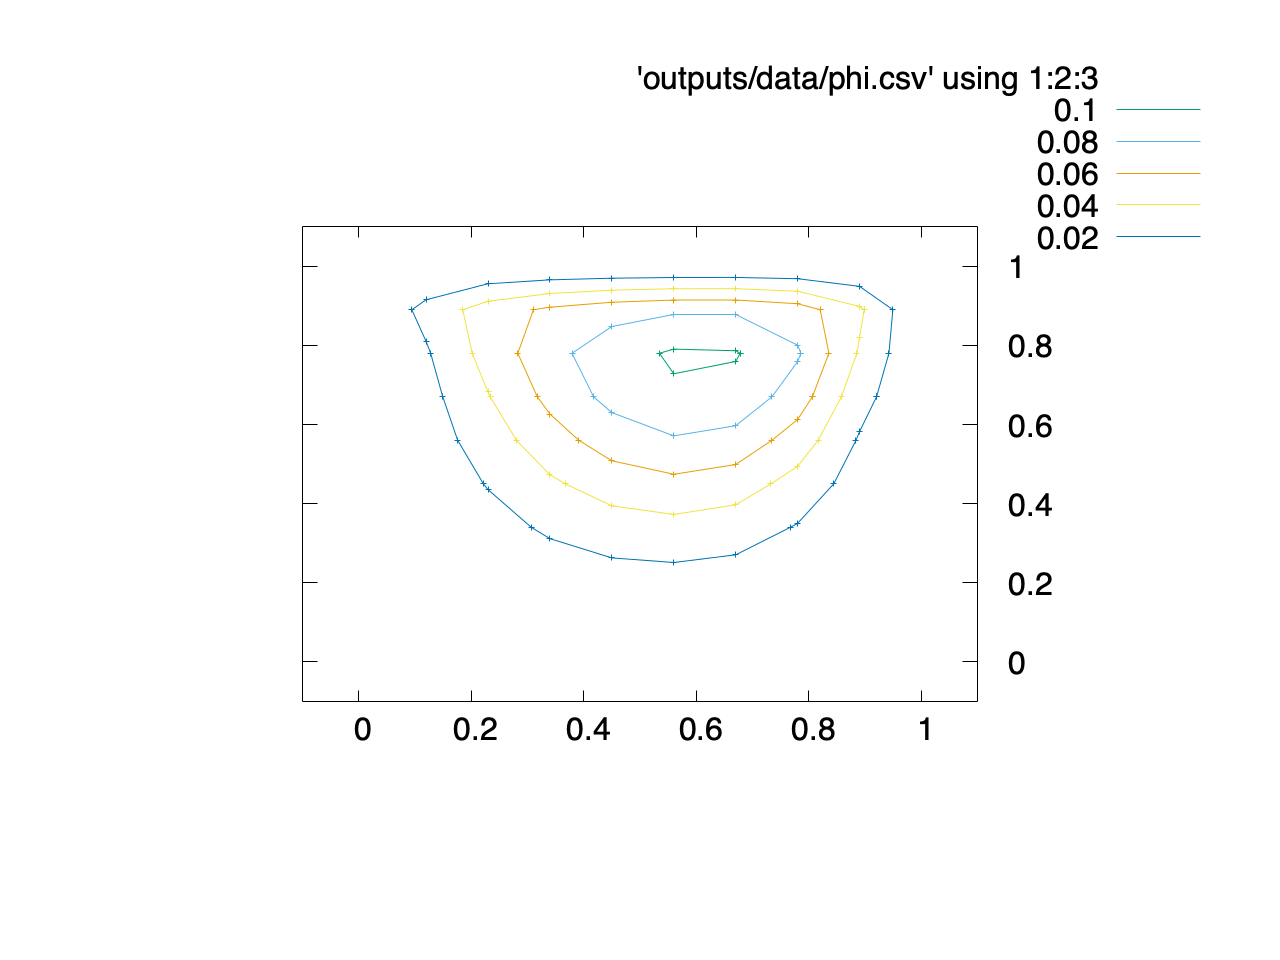
\includegraphics[height=9.5cm]{outputs/img/stream_line.png}
  \caption{流線(dgrid3dパラメータ調整あり)}
  \label{fig:stream_line}
\end{figure}
\section{これから取り組むこと}
\subsection{等圧線図の描画}
圧力のポアソン方程式等により圧力分布を求め,等圧線図を描画する.

\subsection{コードの修正}
同じ処理を複数回記述していたり、可読性に欠ける箇所があるので,関数,モジュールを用いることができるか検討する.

\begin{thebibliography}{9}
  %	\bibitem{1} \url{http://www.hal.t.u-tokyo.ac.jp/lab/ja/index_1.xhtml}
  %    \bibitem{2}Olga Russakovsky*, Jia Deng*, Hao Su, Jonathan Krause, Sanjeev Satheesh, Sean Ma, Zhiheng Huang, Andrej Karpathy, Aditya Khosla, Michael Bernstein, Alexander C. Berg and Li Fei-Fei. (* = equal contribution) ImageNet Large Scale Visual Recognition Challenge. IJCV, 2015.
  \bibitem{1} 研究室資料.流体の数値計算(川口光年先生1976年頃).pdf
  \bibitem{2} Shigeharu TAKENO."gnuplot 34.13 Dgrid3d".2003/10/21.http://takeno.iee.niit.ac.jp/\textasciitilde foo/gp-jman/data/gp372-jp-l2h/node82.html(参照2021/5/31)

\end{thebibliography}

\end{document}